\chapter{Chimie des hétérocycles}\label{ch:b3:heterocycles}

Une tasse de café contient de la caféine, faite de deux cycles accolés qui
renferment quatre atomes d'azote, et son arôme provient de dizaines de
furanes, de pyrroles, de pyrazines et de thiophènes formés à la torréfaction.
La plupart des médicaments d'une officine contiennent au moins un cycle
comportant un atome d'azote, d'oxygène ou de soufre, tout comme les bases
de l'ADN, l'\omterm{def:b3:bioinorganic:haem}{hème} et la chlorophylle, et de nombreuses vitamines. Ce
chapitre explique comment un hétéroatome dans un cycle aromatique modifie
ses électrons~: il peut rendre le cycle plus pauvre ou plus riche que le
benzène, et cela décide du lieu et du mode de sa réactivité. Il se termine
par trois méthodes classiques de construction de ces cycles.

\begin{recall}
Le volume de deuxième année a traité de l'aromaticité et de la règle de
Hückel, des arènes et de la substitution électrophile aromatique via
l'intermédiaire de Wheland, des groupes activants et orienteurs, des amines
et de leur basicité, des imines, des énamines, des tautomères et des bases
nucléiques~; le volume de première année, du $\mathrm pK_a$, des nucléophiles,
des électrophiles et des groupes partants. Le \cref{ch:b3:pericyclic} a
donné le \omterm{def:b3:pericyclic:families}{réarrangement sigmatropique} [3,3].
\end{recall}

\begin{omfigure}
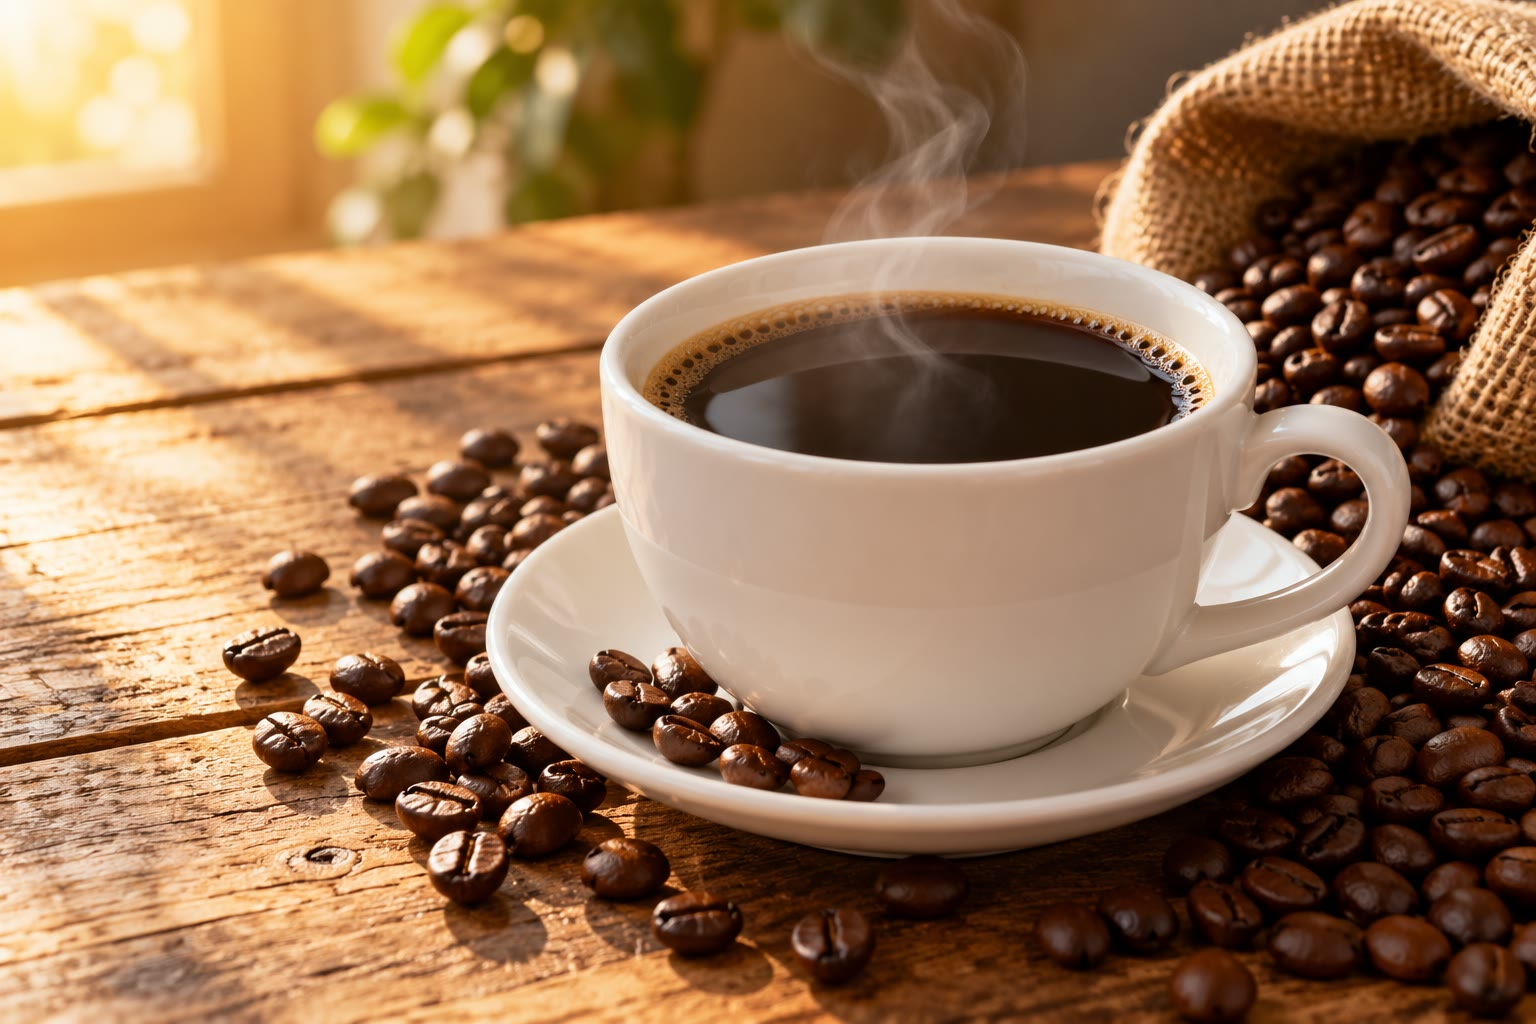
\includegraphics[width=0.5\linewidth]{images/book4/ai/b3-29-coffee.jpg}

{\small Une tasse de café et des grains torréfiés~: la caféine, une purine,
et bon nombre des molécules d'arôme formées à la torréfaction sont des
\omterm{def:b3:heterocycles:heterocycle}{hétérocycles}.}
\end{omfigure}

\section{Hétérocycles aromatiques}

\begin{definition}[Hétérocycles]\label{def:b3:heterocycles:heterocycle}
Un \emph{hétérocycle}\index{heterocycle@hétérocycle} est un composé cyclique comportant dans le
cycle au moins un atome autre que le carbone~; un \emph{composé hétéroaromatique}\index{compose heteroaromatique@composé hétéroaromatique} est un hétérocycle aromatique, comme la
pyridine, le pyrrole, le furane ou le thiophène.
\end{definition}

\begin{proposition}[Six électrons $\pi$]\label{prop:b3:heterocycles:sextet}
La pyridine, le pyrrole, le furane, le thiophène et l'imidazole possèdent chacun six électrons $\pi$ dans
un système plan, cyclique et conjugué, et sont aromatiques d'après la règle
de Hückel.
\end{proposition}

\begin{proof}
Pyridine~: les cinq carbones et l'azote apportent chacun un électron p~; le
doublet de l'azote est dans une orbitale $sp^2$ du plan du cycle, hors du système $\pi$~: $5 + 1 = 6$.
Pyrrole~: les quatre carbones en apportent un chacun et l'azote, lié à H
dans le plan, place son doublet dans son orbitale p~: $4 + 2 = 6$. Furane et thiophène~: comme le
pyrrole, l'hétéroatome apportant l'un de ses deux doublets (l'autre est
dans le plan). Imidazole~: l'azote N--H en apporte deux, l'azote de type
pyridine un, les trois carbones trois~: 6. Six vaut $4n + 2$ avec $n = 1$.
\end{proof}

\begin{omfigure}
\begin{tikzpicture}[font=\small, yscale=0.55]
  % pyridine: six p orbitals perpendicular to the ring (drawn first), N at 0 deg
  \foreach \a in {0,60,...,300} { \pic at (\a:1.1) {omp={0.62}{90}}; }
  \draw[thick] (0:1.1) -- (60:1.1) -- (120:1.1) -- (180:1.1) -- (240:1.1) -- (300:1.1) -- cycle;
  \node[fill=white, inner sep=0.5pt] at (0:1.1) {N};
  \pic at ($(0:1.1)+(0.2,0)$) {omlobe={0.8}{0}};
  \node[font=\scriptsize, align=center, anchor=north] at (0,-2.4) {pyridine~: 6 électrons p issus de 6 atomes~;\\ doublet dans le plan (basique)};
  \begin{scope}[xshift=5.4cm]
    \foreach \a in {0,72,144,216,288} { \pic at (\a:1.0) {omp={0.62}{90}}; }
    \draw[thick] (0:1.0) -- (72:1.0) -- (144:1.0) -- (216:1.0) -- (288:1.0) -- cycle;
    \node[fill=white, inner sep=0.5pt] at (0:1.0) {N};
    \draw ($(0:1.0)+(0.18,0)$) -- (0:1.7) node[right, inner sep=0.5pt] {H};
    \node[font=\scriptsize, align=center, anchor=north] at (0,-2.4) {pyrrole~: le doublet de N est l'un\\ des 6 électrons $\pi$ (non basique)};
  \end{scope}
\end{tikzpicture}

{\small Les systèmes $\pi$ de la pyridine et du pyrrole, vus en oblique~: une orbitale p par
atome du cycle, perpendiculaire au cycle. Dans la pyridine, le doublet de
l'azote (le lobe situé dans le plan, sur l'azote) pointe vers l'extérieur
dans le plan du cycle et peut fixer un proton~; dans le pyrrole, l'azote,
qui porte un hydrogène dans le plan, cède son doublet au sextet
aromatique.}
\end{omfigure}

\begin{definition}[Hétérocycles $\pi$-excédentaires et $\pi$-déficitaires]\label{def:b3:heterocycles:pi-character}
Un \emph{hétérocycle $\pi$-excédentaire}\index{heterocycle pi-excedentaire@hétérocycle $\pi$-excédentaire}, comme le
pyrrole, le furane ou le thiophène, a six électrons $\pi$ sur cinq atomes et une \omterm{def:b3:computational-chemistry:dft}{densité
électronique} $\pi$ sur ses carbones plus élevée que celle du benzène~; un \emph{hétérocycle $\pi$-déficitaire}\index{heterocycle pi-deficitaire@hétérocycle $\pi$-déficitaire}, comme la pyridine, possède un
atome électronégatif dans le cycle qui attire la densité $\pi$ hors des carbones.
\end{definition}

\begin{proposition}[Basicité]\label{prop:b3:heterocycles:basicity}
La pyridine est une base moyenne et le pyrrole n'est presque pas basique~;
le pyrrole, lorsqu'il est protoné en milieu acide fort, prend le proton sur
un carbone, non sur l'azote.
\end{proposition}

\begin{proof}[Justification]
% ledger: pka:pyridinium, pka4:pyrrolium, pka4:piperidinium, pka4:imidazolium, pka4:DMAPH
Le doublet de la pyridine est hors du système $\pi$~: le protoner ne coûte
aucune aromaticité, et le pyridinium a un $\mathrm pK_a = 5.2$~; la pyridine est moins basique que la pipéridine
(l'azote du pyridinium est $sp^2$, avec plus de caractère s, et retient plus
fortement son doublet~: pipéridinium 11.1). Protoner l'azote du pyrrole
retirerait son doublet du sextet et détruirait l'aromaticité~; seuls des
acides très forts protonent le pyrrole, en C2, où le cation conserve une
certaine délocalisation
($\mathrm pK_a$ d'environ $-4$). L'imidazole possède les deux sortes d'azote~: il est protoné sur
l'azote de type pyridine, et son cation, symétrique, est stabilisé par résonance ($\mathrm pK_a$
7.0), ce qui explique que l'histidine fonctionne comme acide et comme base
dans les \omterm{def:b3:complex-kinetics:enzyme}{enzymes}. La 4-(diméthylamino)pyridine est plus basique encore ($\mathrm pK_a$ 9.6)~: le groupe amino pousse
son doublet dans le cycle et jusque sur l'azote du cycle.
\end{proof}

% ledger: dip:pyridine, dip4:pyrrole, dip4:furan, dip4:thiophene
Les moments dipolaires racontent la même histoire~: la pyridine (\qty{2.19}{D}) a son
extrémité négative sur l'azote, alors que dans le pyrrole (\qty{1.84}{D}) la cession du doublet au
cycle place l'extrémité négative sur le cycle et l'extrémité positive sur
l'azote. Dans le furane
(\qty{0.66}{D}) et le thiophène (\qty{0.55}{D}), les deux effets, attraction $\sigma$ et donation $\pi$, se
compensent presque.

\begin{omfigure}
% ledger: h1:pyridine.a, h1:pyridine.g, h1:pyridine.b, h1:pyrrole.a, h1:pyrrole.b, h1:pyrrole.NH, h1:furan.a, h1:furan.b
\begin{tikzpicture}
\begin{axis}[width=0.86\linewidth, height=6.2cm, x dir=reverse, xmin=5.8, xmax=9.0, ymin=-0.1, ymax=3.6,
  axis x line=bottom, axis y line=none, xlabel={$\delta$ / ppm}, tick label style={font=\scriptsize}, label style={font=\small}]
\addplot[omDef, thick] table[x=ppm, y expr=\thisrow{y}+2.4] {figdata/out/bachelor-3-heterocycle-nmr-pyridine.dat};
\addplot[omThm, thick] table[x=ppm, y expr=\thisrow{y}+1.2] {figdata/out/bachelor-3-heterocycle-nmr-pyrrole.dat};
\addplot[omMeth, thick] table[x=ppm, y=y] {figdata/out/bachelor-3-heterocycle-nmr-furan.dat};
\node[font=\scriptsize, omDef, anchor=east] at (axis cs:5.82,3.0) {pyridine~: H2/6, H4, H3/5 (2\,:\,1\,:\,2)};
\node[font=\scriptsize, omThm, anchor=west] at (axis cs:7.7,1.8) {pyrrole~: NH, H2/5, H3/4};
\node[font=\scriptsize, omMeth, anchor=west] at (axis cs:7.2,0.6) {furane~: H2/5, H3/4};
\end{axis}
\end{tikzpicture}

{\small RMN du proton de la pyridine, du pyrrole et du furane dans le
chloroforme deutéré, synthétisée à partir de déplacements mesurés sous
forme de raies simples (couplages omis), d'aires égales aux nombres de
protons. La pyridine, $\pi$-déficitaire, a ses signaux H2/6 et H4
nettement déblindés par rapport à celui du benzène~; le pyrrole et le
furane, $\pi$-excédentaires, ont la plupart des leurs blindés par rapport à
lui~; les protons voisins de l'hétéroatome sont toujours les plus
déblindés.}
\end{omfigure}

\section{La pyridine}

La pyridine résiste à la substitution électrophile~: l'électrophile
rencontre un cycle plus pauvre en électrons que le benzène et, dans l'acide
habituellement présent, un ion pyridinium dont la charge positive le
repousse. La nitration exige des conditions très dures et donne
l'isomère 3 avec un faible rendement.

\begin{proposition}[Substitution électrophile en C3]\label{prop:b3:heterocycles:pyridine-c3}
L'attaque électrophile sur la pyridine a lieu en C3~: l'attaque en C2 ou en
C4 donne un intermédiaire de Wheland dont l'une des formes mésomères place
la charge positive sur un azote entouré de six électrons seulement.
\end{proposition}

\begin{proof}
Dans le cation issu de l'attaque en C2 (ou en C4), la charge positive se
répartit sur C3, C5 et N1 (ou sur C3, C5 et N1)~: une forme mésomère
comporte un azote déficitaire, à six électrons, très défavorable pour un
atome électronégatif. L'attaque en C3 répartit la charge sur C2, C4 et C6
seulement. Les trois cations sont tous moins stables que celui du benzène,
mais l'attaque en C3 est la moins défavorable.
\end{proof}

\begin{definition}[N-oxyde de pyridine]\label{def:b3:heterocycles:n-oxide}
Un \emph{N-oxyde de pyridine}\index{N-oxyde de pyridine}, obtenu en oxydant la pyridine
par un peroxyacide, possède un groupe $\mathrm{N^+{-}O^-}$ dont l'oxygène rend des électrons à C2
et à C4~; il subit la substitution électrophile en C4, et l'oxygène est
ensuite éliminé.
\end{definition}

\begin{definition}[Substitution nucléophile aromatique]\label{def:b3:heterocycles:snar}
La \emph{substitution nucléophile aromatique}\index{substitution nucleophile aromatique@substitution nucléophile aromatique}
($\mathrm S_\mathrm NAr$) remplace un groupe partant porté par un cycle aromatique pauvre en
électrons par un nucléophile, par addition puis élimination. L'intermédiaire
d'addition anionique est un \emph{complexe de Meisenheimer}\index{complexe de Meisenheimer}.
\end{definition}

\begin{proposition}[$\mathrm S_\mathrm NAr$ en C2 et en C4]\label{prop:b3:heterocycles:snar-positions}
Les halogénopyridines subissent facilement la $\mathrm S_\mathrm NAr$ en C2 et en C4 et seulement difficilement en C3,
parce que l'addition en C2 ou en C4 place la charge négative sur l'azote.
\end{proposition}

\begin{proof}
L'addition en C2 rend C2 $sp^3$ et laisse quatre électrons $\pi$ plus le doublet entrant
répartis sur N1, C3 et C5 (ou, pour C4~: C3, C5 et N1)~: une forme mésomère
place la charge négative sur l'azote électronégatif. L'addition en C3 la
répartit sur C2, C4 et C6 seulement, tous des carbones.
\end{proof}

\begin{omfigure}
\begin{tikzpicture}[font=\small, >=Stealth]
  \draw[thick] (-0.000,-0.620) -- (0.537,-0.310) -- (0.537,0.310) -- (0.000,0.620) -- (-0.537,0.310) -- (-0.537,-0.310) -- cycle;
  \draw[thick] (0.082,-0.424) -- (0.326,-0.283);
  \draw[thick] (0.326,0.283) -- (0.082,0.424);
  \draw[thick] (-0.408,0.141) -- (-0.408,-0.141);
  \node[fill=white, inner sep=0.4pt, font=\scriptsize] at (-0.000,-0.620) {N};
  \draw (0.537,-0.310) -- (0.927,-0.535) node[right, inner sep=0.5pt, font=\scriptsize] {Cl};
  \draw[thick] (3.400,-0.620) -- (3.937,-0.310) -- (3.937,0.310) -- (3.400,0.620) -- (2.863,0.310) -- (2.863,-0.310) -- cycle;
  \draw[thick] (3.726,0.283) -- (3.482,0.424);
  \draw[thick] (2.992,0.141) -- (2.992,-0.141);
  \node[fill=white, inner sep=0.4pt, font=\scriptsize] at (3.400,-0.620) {N};
  \node[font=\scriptsize, omThm] at (3.350,-0.920) {$\ominus$};
  \draw (3.937,-0.310) -- (4.386,-0.343) node[right, inner sep=0.5pt, font=\scriptsize] {Nu};
  \draw (3.937,-0.310) -- (4.190,-0.682) node[right, inner sep=0.5pt, font=\scriptsize] {Cl};
  \draw[thick] (6.800,-0.620) -- (7.337,-0.310) -- (7.337,0.310) -- (6.800,0.620) -- (6.263,0.310) -- (6.263,-0.310) -- cycle;
  \draw[thick] (6.882,-0.424) -- (7.126,-0.283);
  \draw[thick] (7.126,0.283) -- (6.882,0.424);
  \draw[thick] (6.392,0.141) -- (6.392,-0.141);
  \node[fill=white, inner sep=0.4pt, font=\scriptsize] at (6.800,-0.620) {N};
  \draw (7.337,-0.310) -- (7.727,-0.535) node[right, inner sep=0.5pt, font=\scriptsize] {Nu};
  \draw[->, thick] (1.25,0) -- (2.35,0) node[midway, above, font=\scriptsize] {$+\,\mathrm{Nu^-}$};
  \draw[->, thick] (4.65,0) -- (5.75,0) node[midway, above, font=\scriptsize] {$-\,\ce{Cl-}$};
  \node[font=\scriptsize] at (3.4,-1.2) {complexe de Meisenheimer};
\end{tikzpicture}

{\small Substitution nucléophile de la 2-chloropyridine~: le nucléophile
s'additionne sur C2, ce qui donne un intermédiaire anionique dont la charge
négative se trouve en grande partie sur l'azote du cycle (une forme
mésomère représentée)~; le chlorure part ensuite et le cycle aromatique est
restauré.}
\end{omfigure}

\begin{proposition}[Addition--élimination]\label{prop:b3:heterocycles:snar-mechanism}
Pour une réaction de $\mathrm S_\mathrm NAr$ dont l'étape d'addition est cinétiquement déterminante, $v = k[\mathrm{ArX}][\mathrm{Nu^-}]$,
et le fluorure est le meilleur groupe partant parmi les halogénures.
\end{proposition}

\begin{proof}[Justification]
La vitesse est celle de l'addition bimoléculaire. La liaison
carbone--halogène n'est pas rompue au cours de cette étape~; ce qui compte,
c'est à quel point l'halogène abaisse l'énergie de l'état de transition
anionique en attirant les électrons, et le fluor, le plus électronégatif,
le fait le plus~: d'où l'ordre F $>$ Cl $\approx$ Br $>$ I, inverse de celui de la $\mathrm S_\mathrm N2$.
\end{proof}

\begin{definition}[Réaction de Tchitchibabine]\label{def:b3:heterocycles:chichibabin}
La \emph{réaction de Tchitchibabine}\index{reaction de Tchitchibabine@réaction de Tchitchibabine} est l'amination de
la pyridine en C2 par l'amidure de sodium~: l'ion amidure s'additionne sur
C2, et un ion hydrure est perdu, sous forme de dihydrogène après réaction
avec le produit.
\end{definition}

La pyridine et la DMAP servent aussi de bases et de catalyseurs
nucléophiles~: dans les acylations par les anhydrides d'acide, la DMAP
attaque d'abord l'anhydride, ce qui donne un ion acylpyridinium qui
transfère son groupe acyle à l'alcool bien plus vite que l'anhydride
lui-même. Les pyridines, les bipyridines et les phénanthrolines comptent
parmi les ligands les plus courants de la chimie de coordination.

\section{Cycles à cinq chaînons}

\begin{proposition}[Substitution électrophile du pyrrole en C2]\label{prop:b3:heterocycles:pyrrole-c2}
Le pyrrole, le furane et le thiophène subissent la substitution
électrophile principalement en C2, parce que le cation issu de l'attaque en
C2 possède trois formes mésomères et celui issu de l'attaque en C3
seulement deux.
\end{proposition}

\begin{proof}
Après une attaque en C2, la charge positive peut se trouver sur C3, sur C5
ou sur l'azote, où elle est partagée grâce au doublet et où chaque atome
garde un octet (troisième forme). Après une attaque en C3, elle ne peut se
trouver que sur C2 ou sur l'azote~: la charge est moins délocalisée (voir la
figure).
\end{proof}

\begin{omfigure}
\begin{tikzpicture}[font=\small]
  \draw[thick] (0.000,0.620) -- (0.590,0.192) -- (0.364,-0.502) -- (-0.364,-0.502) -- (-0.590,0.192) -- cycle;
  \draw[thick] (-0.303,-0.269) -- (-0.403,0.039);
  \node[fill=white, inner sep=0.4pt, font=\scriptsize] at (0.000,0.620) {N};
  \draw (0.000,0.750) -- (0.000,1.020) node[above, inner sep=0.5pt, font=\scriptsize] {H};
  \draw (0.590,0.192) -- (0.893,0.482) node[right, inner sep=0.5pt, font=\scriptsize] {H};
  \draw (0.590,0.192) -- (1.006,0.135) node[right, inner sep=0.5pt, font=\scriptsize] {E};
  \node[font=\scriptsize, omThm] at (0.164,-0.226) {$\oplus$};
  \draw[thick] (2.600,0.620) -- (3.190,0.192) -- (2.964,-0.502) -- (2.236,-0.502) -- (2.010,0.192) -- cycle;
  \draw[thick] (2.762,-0.371) -- (2.438,-0.371);
  \node[fill=white, inner sep=0.4pt, font=\scriptsize] at (2.600,0.620) {N};
  \draw (2.600,0.750) -- (2.600,1.020) node[above, inner sep=0.5pt, font=\scriptsize] {H};
  \draw (3.190,0.192) -- (3.493,0.482) node[right, inner sep=0.5pt, font=\scriptsize] {H};
  \draw (3.190,0.192) -- (3.606,0.135) node[right, inner sep=0.5pt, font=\scriptsize] {E};
  \node[font=\scriptsize, omThm] at (2.335,0.086) {$\oplus$};
  \draw[thick] (5.200,0.620) -- (5.790,0.192) -- (5.564,-0.502) -- (4.836,-0.502) -- (4.610,0.192) -- cycle;
  \draw[thick] (5.362,-0.371) -- (5.038,-0.371);
  \draw[thick] (5.113,0.395) -- (4.851,0.205);
  \node[fill=white, inner sep=0.4pt, font=\scriptsize] at (5.200,0.620) {N};
  \draw (5.200,0.750) -- (5.200,1.020) node[above, inner sep=0.5pt, font=\scriptsize] {H};
  \draw (5.790,0.192) -- (6.093,0.482) node[right, inner sep=0.5pt, font=\scriptsize] {H};
  \draw (5.790,0.192) -- (6.206,0.135) node[right, inner sep=0.5pt, font=\scriptsize] {E};
  \node[font=\scriptsize, omThm] at (5.480,0.700) {$\oplus$};
  \draw[thick] (8.400,0.620) -- (8.990,0.192) -- (8.764,-0.502) -- (8.036,-0.502) -- (7.810,0.192) -- cycle;
  \draw[thick] (8.097,-0.269) -- (7.997,0.039);
  \node[fill=white, inner sep=0.4pt, font=\scriptsize] at (8.400,0.620) {N};
  \draw (8.400,0.750) -- (8.400,1.020) node[above, inner sep=0.5pt, font=\scriptsize] {H};
  \draw (8.764,-0.502) -- (9.135,-0.700) node[right, inner sep=0.5pt, font=\scriptsize] {H};
  \draw (8.764,-0.502) -- (8.839,-0.915) node[right, inner sep=0.5pt, font=\scriptsize] {E};
  \node[font=\scriptsize, omThm] at (8.665,0.086) {$\oplus$};
  \draw[thick] (11.000,0.620) -- (11.590,0.192) -- (11.364,-0.502) -- (10.636,-0.502) -- (10.410,0.192) -- cycle;
  \draw[thick] (10.697,-0.269) -- (10.597,0.039);
  \draw[thick] (11.087,0.395) -- (11.349,0.205);
  \node[fill=white, inner sep=0.4pt, font=\scriptsize] at (11.000,0.620) {N};
  \draw (11.000,0.750) -- (11.000,1.020) node[above, inner sep=0.5pt, font=\scriptsize] {H};
  \draw (11.364,-0.502) -- (11.735,-0.700) node[right, inner sep=0.5pt, font=\scriptsize] {H};
  \draw (11.364,-0.502) -- (11.439,-0.915) node[right, inner sep=0.5pt, font=\scriptsize] {E};
  \node[font=\scriptsize, omThm] at (11.280,0.700) {$\oplus$};
  \node[font=\scriptsize] at (2.6,-1.35) {attaque en C2~: trois formes mésomères};
  \node[font=\scriptsize] at (9.7,-1.35) {attaque en C3~: deux formes mésomères};
  \draw[black!40] (6.8,-1.2) -- (6.8,1.2);
\end{tikzpicture}

{\small Intermédiaires de Wheland du pyrrole (E~: l'électrophile~; $\oplus$~: charge positive).
L'attaque en C2 donne un cation dont la charge est sur C3, sur C5 ou sur
l'azote, tous les octets étant complets~; l'attaque en C3, sur C2 ou sur
l'azote seulement.}
\end{omfigure}

Le pyrrole est à peu près aussi réactif que le phénol ou l'aniline~: il est
bromé, nitré et acylé dans des conditions douces, polymérise en milieu
acide fort, et est formylé en C2 par le réactif de Vilsmeier issu du
diméthylformamide et du chlorure de phosphoryle. Les réactivités décroissent dans l'ordre pyrrole $>$ furane $>$ thiophène $>$ benzène,
suivant la disposition de l'hétéroatome à partager son doublet. Le furane,
le moins aromatique, réagit aussi comme diène dans les réactions de
Diels--Alder. Les bases fortes comme le butyllithium déprotonent le furane
et le thiophène en C2, à côté de l'hétéroatome, ce qui donne des
organolithiens.

\begin{method}[Prévoir le site d'attaque sur un hétérocycle]\label{met:b3:heterocycles:site}
\begin{enumerate}
  \item Classer le cycle~: $\pi$-excédentaire (hétéroatome de type pyrrole) ou $\pi$-déficitaire
        (azote de type pyridine).
  \item Électrophiles~: sur un cycle $\pi$-excédentaire en C2 (en C3 pour l'indole, dont l'attaque en C2
        perturberait le cycle benzénique)~; sur la pyridine en C3, ou en C4 via
        le N-oxyde.
  \item Nucléophiles~: sur un cycle $\pi$-déficitaire en C2 ou en C4, surtout si un groupe
        partant s'y trouve.
  \item Bases fortes~: sur la liaison C--H voisine de l'hétéroatome.
\end{enumerate}
\end{method}

\section{Hétérocycles condensés et biologiques}

L'indole, un benzène accolé à un pyrrole, réagit avec les électrophiles en
C3~: l'intermédiaire y conserve intact le cycle benzénique, la charge étant
sur l'azote. La quinoléine, un benzène accolé à une pyridine, est
substituée par les électrophiles sur son cycle benzénique et par les
nucléophiles en C2 et en C4. Les bases nucléiques sont des pyrimidines
(cytosine, thymine, uracile) et des purines (adénine, guanine), une
pyrimidine accolée à un imidazole. Leurs formes oxo et amino (tautomères
lactame et amine) l'emportent sur les formes hydroxy et imino, ce qui fixe
la disposition des donneurs et des accepteurs de liaison hydrogène sur
chaque base, et donc l'appariement des bases.

\begin{omfigure}
\begin{tikzpicture}[font=\small]
  \node[draw, rounded corners, minimum width=1.8cm, minimum height=2.8cm, fill=omDef!8] at (0,0) {};
  \node[font=\small\bfseries] at (0,1.75) {guanine};
  \node[anchor=east] (g1) at (0.85,0.85) {C6=O};
  \node[anchor=east] (g2) at (0.85,0) {N1--H};
  \node[anchor=east] (g3) at (0.85,-0.85) {C2--N--H};
  \node[draw, rounded corners, minimum width=1.8cm, minimum height=2.8cm, fill=omThm!8] at (3.2,0) {};
  \node[font=\small\bfseries] at (3.2,1.75) {cytosine};
  \node[anchor=west] (c1) at (2.35,0.85) {H--N--C4};
  \node[anchor=west] (c2) at (2.35,0) {N3};
  \node[anchor=west] (c3) at (2.35,-0.85) {O=C2};
  \draw[omMeth, very thick, dotted] (g1.east) -- (c1.west);
  \draw[omMeth, very thick, dotted] (g2.east) -- (c2.west);
  \draw[omMeth, very thick, dotted] (g3.east) -- (c3.west);
\end{tikzpicture}

{\small Une paire de bases guanine--cytosine, schématique~: trois liaisons
hydrogène (en vert) entre l'oxygène du carbonyle de la guanine et un N--H
amino de la cytosine, le N1--H de la guanine et le N3 du cycle de la
cytosine, et un N--H amino de la guanine et l'oxygène du carbonyle de la
cytosine. L'adénine et la thymine en forment deux.}
\end{omfigure}

\section{Construire des cycles}

\begin{definition}[Synthèse de Paal--Knorr]\label{def:b3:heterocycles:paal-knorr}
La \emph{synthèse de Paal--Knorr}\index{synthese de Paal--Knorr@synthèse de Paal--Knorr} prépare un furane
(avec un acide), un pyrrole (avec une amine primaire ou l'ammoniac) ou un
thiophène (avec un réactif soufré) à partir d'un composé 1,4-dicarbonylé.
\end{definition}

\begin{definition}[Synthèse des pyridines de Hantzsch]\label{def:b3:heterocycles:hantzsch}
La \emph{synthèse des pyridines de Hantzsch}\index{synthese des pyridines de Hantzsch@synthèse des pyridines de Hantzsch}
condense un aldéhyde, deux équivalents d'un $\beta$-cétoester et l'ammoniac en une
1,4-dihydropyridine, qui peut être oxydée en pyridine.
\end{definition}

\begin{definition}[Synthèse des indoles de Fischer]\label{def:b3:heterocycles:fischer-indole}
La \emph{synthèse des indoles de Fischer}\index{synthese des indoles de Fischer@synthèse des indoles de Fischer} chauffe la
phénylhydrazone d'un aldéhyde ou d'une cétone avec un catalyseur acide~:
l'hydrazone se tautomérise en ène-hydrazine, qui subit un \omterm{def:b3:pericyclic:families}{réarrangement
sigmatropique} [3,3]~; une cyclisation et la perte d'ammoniac donnent
l'indole.
\end{definition}

\begin{omfigure}
\setchemfig{atom sep=1.8em}
\schemestart
\chemfig{*6(-=-=(-NH-[:30]N=[:-30](-[:-90]CH_3)-[:30]CH_3)-=)}
\arrow{->[$\ce{H+}$][tautomérie]}[,1.4]
\chemfig{*6(-=-=(-NH-[:30]NH-[:-30](=[:-90]CH_2)-[:30]CH_3)-=)}
\schemestop
\par\bigskip
\schemestart
\arrow{->[{[3,3]}, puis][cyclisation, $-\ce{NH3}$]}[,2.2]
\chemfig{*6(-=*5(-=(-CH_3)-N(-H)-)-=-=)}
\schemestop

{\small La \omterm{def:b3:heterocycles:fischer-indole}{synthèse des indoles de Fischer} à partir de la phénylhydrazone de
l'acétone. L'acide transforme l'hydrazone en son tautomère ène-hydrazine~;
le réarrangement [3,3] rompt la liaison N--N et forme une liaison C--C entre
le carbone du cycle en \textit{ortho} de l'azote et le
$\ce{CH2}$ terminal~; la nouvelle amine attaque l'imine, et la perte d'ammoniac donne le
2-méthylindole.}
\end{omfigure}

\begin{method}[Déconnecter un hétérocycle]\label{met:b3:heterocycles:disconnect}
\begin{enumerate}
  \item Un pyrrole, un furane ou un thiophène 2,5-disubstitué~: déconnecter
        les deux liaisons à l'hétéroatome, pour revenir à une 1,4-dicétone
        (Paal--Knorr).
  \item Une 1,4-dihydropyridine symétrique portant des esters en C3 et en C5~: revenir à un
        aldéhyde, deux $\beta$-cétoesters et l'ammoniac (Hantzsch).
  \item Un indole 2,3-disubstitué~: revenir à la phénylhydrazine et à la
        cétone
        $\mathrm{R^2CH_2COR^3}$ (Fischer).
  \item Vérifier la disponibilité des fragments, puis la régiochimie
        lorsque la cétone n'est pas symétrique.
\end{enumerate}
\end{method}

\begin{definition}[Bioisostère]\label{def:b3:heterocycles:bioisostere}
Un \emph{bioisostère}\index{bioisostere@bioisostère} est un groupe qui en remplace un autre dans une
molécule de médicament en conservant son activité biologique, parce qu'il
a une taille, une forme et une disposition des liaisons hydrogène et des
charges semblables, comme un tétrazole à la place d'un acide carboxylique,
ou une pyridine à la place d'un cycle benzénique.
\end{definition}

\begin{inthelab}[Un pyrrole de Paal--Knorr]
L'hexane-2,5-dione, l'aniline et une quantité catalytique d'acide
4-toluènesulfonique sont chauffées à reflux dans le toluène dans un ballon
muni d'un appareil de Dean--Stark~: l'eau formée est entraînée sous forme
d'azéotrope et se rassemble dans le bras latéral, ce qui rend la
condensation totale. Lorsque l'eau ne se sépare plus, la solution est lavée
par une solution aqueuse d'hydrogénocarbonate de sodium, séchée et
évaporée, et le 2,5-diméthyl-1-phénylpyrrole est recristallisé.
\end{inthelab}

\begin{safety}{\ghs[0.62cm]{GHS02}\ghs[0.62cm]{GHS06}\ghs[0.62cm]{GHS07}\ghs[0.62cm]{GHS08}\ghs[0.62cm]{GHS09}}
% ledger: ghs4:pyridine, ghs4:phenylhydrazine
Pyridine~: très inflammable, nocive par toutes les voies d'exposition, à
l'odeur forte~; utilisée sous une hotte. Phénylhydrazine~: toxique par
toutes les voies d'exposition, peut provoquer le cancer et des anomalies
génétiques, altère le sang en cas d'exposition répétée, sensibilisante,
très toxique pour les organismes aquatiques~; elle est pesée sous une hotte
avec des gants, et ses déchets sont collectés séparément.
\end{safety}

\begin{history}[Deux synthèses de cycles classiques]
Emil Fischer décrivit sa synthèse des indoles en 1883, dans les années de
ses travaux sur les sucres et les purines~; Arthur Hantzsch publia sa
synthèse des pyridines en 1881. Les deux restent utilisées~: la synthèse de
Fischer pour les triptans contre la migraine, la synthèse de Hantzsch pour
les dihydropyridines inhibitrices calciques qui traitent l'hypertension
artérielle.
\end{history}

\section{Exercices}

\begin{exercise}[$\star$]\label{exo:b3:heterocycles:1}
Dénombrer les électrons $\pi$ de l'oxazole, du thiazole, de la pyrimidine et de la purine, et dire quels
doublets appartiennent au système $\pi$.
\end{exercise}

\begin{exercise}[$\star$]\label{exo:b3:heterocycles:2}
Classer la pyridine, le pyrrole, l'imidazole, la pipéridine et la DMAP par
basicité, avec leurs valeurs de
$\mathrm pK_a$.
\end{exercise}

\begin{exercise}[$\star$]\label{exo:b3:heterocycles:3}
Donner le produit principal de la monobromation du pyrrole, du furane et de l'indole.
\end{exercise}

\begin{exercise}[$\star$]\label{exo:b3:heterocycles:4}
Donner les produits de la réaction de Paal--Knorr de l'hexane-2,5-dione avec
un acide seul, avec la méthylamine, et avec le pentasulfure de phosphore.
\end{exercise}

\begin{exercise}[$\star\star$]\label{exo:b3:heterocycles:5}
La 2-chloropyridine réagit avec le méthanolate de sodium dans le méthanol à \qty{65}{\celsius}~; la 3-chloropyridine
réagit à peine. Expliquer, et donner le produit.
\end{exercise}

\begin{exercise}[$\star\star$]\label{exo:b3:heterocycles:6}
Donner le produit de la \omterm{def:b3:heterocycles:chichibabin}{réaction de Tchitchibabine} de la pyridine et
dessiner l'intermédiaire d'addition.
\end{exercise}

\begin{exercise}[$\star\star$]\label{exo:b3:heterocycles:7}
Le \omterm{def:b3:heterocycles:n-oxide}{N-oxyde de pyridine} est nitré en C4. L'expliquer à l'aide des formes
mésomères, et dire comment on obtient la 4-nitropyridine.
\end{exercise}

\begin{exercise}[$\star\star$]\label{exo:b3:heterocycles:8}
La 2-hydroxypyridine existe principalement dans l'eau sous forme de
2-pyridone. Dessiner les deux tautomères et expliquer pourquoi la pyridone
est encore aromatique.
\end{exercise}

\begin{exercise}[$\star\star$]\label{exo:b3:heterocycles:9}
Donner les composants d'une synthèse de Hantzsch de la 1,4-dihydropyridine
portant des esters méthyliques en C3 et en C5, des groupes méthyle en C2 et
en C6 et un groupe 2-nitrophényle en C4.
\end{exercise}

\begin{exercise}[$\star\star\star$]\label{exo:b3:heterocycles:10}
La butanone donne deux indoles différents dans la synthèse de Fischer avec
la phénylhydrazine. Donner les deux, et dire comment la force de l'acide
modifie leur rapport.
\end{exercise}

\begin{exercise}[$\star\star\star$]\label{exo:b3:heterocycles:11}
Expliquer pourquoi le 4-fluoronitrobenzène et la 2-fluoropyridine réagissent
avec les nucléophiles plus vite que les chlorures correspondants, contrairement aux substrats de $\mathrm S_\mathrm N2$.
\end{exercise}

\begin{exercise}[$\star\star\star$]\label{exo:b3:heterocycles:12}
À l'aide des spectres synthétiques du chapitre, expliquer comment
distinguer la pyridine, le pyrrole et le furane par leur spectre RMN du
proton, et prévoir le spectre du
thiophène (déplacements \qty{7.33}{ppm} et \qty{7.12}{ppm}).
\end{exercise}

\section{Problème~: construire un indole}

\begin{problem}[{Problème du week-end --- construire un indole~: la
phénylhydrazone de l'acétone, l'ène-hydrazine et son réarrangement [3,3],
la perte d'ammoniac, et le choix entre deux indoles avec la butanone}]
\label{pb:b3:heterocycles:1}
% ledger: aw:C, aw:H, aw:N, aw:O
Données du problème~: 10.0 g de phénylhydrazine réagissent avec un excès
d'acétone, et l'hydrazone est chauffée avec du chlorure de zinc.

\medskip\noindent\textbf{Partie I --- L'hydrazone.}
\begin{enumerate}
  \item Écrire la formation de la phénylhydrazone de l'acétone.
  \item Pourquoi est-ce une condensation de type imine, et pourquoi une
        trace d'acide est-elle utile~?
  \item Quel azote de la phénylhydrazine attaque le groupe carbonyle, et
        pourquoi~?
  \item Calculer la masse molaire de la phénylhydrazine et la quantité
        utilisée.
  \item Calculer la masse théorique d'hydrazone.
\end{enumerate}

\medskip\noindent\textbf{Partie II --- L'ène-hydrazine et l'étape [3,3].}
\begin{enumerate}[resume]
  \item Dessiner le tautomère ène-hydrazine.
  \item Quels six atomes forment l'état de transition cyclique du
        réarrangement [3,3]~?
  \item Quelle liaison se rompt et laquelle se forme~?
  \item Combien d'électrons participent, et l'étape est-elle thermiquement
        permise~?
  \item Quel est le rôle du chlorure de zinc~?
  \item Pourquoi l'aromaticité du cycle benzénique doit-elle être restaurée
        ensuite~?
\end{enumerate}

\medskip\noindent\textbf{Partie III --- La fermeture du cycle.}
\begin{enumerate}[resume]
  \item Quelle amine attaque quel carbone pour fermer le cycle à cinq
        chaînons~?
  \item Quelle petite molécule part, et qu'est-ce qui entraîne la dernière
        étape~?
  \item Écrire l'équation globale, de l'hydrazone au 2-méthylindole.
  \item Calculer la masse molaire du 2-méthylindole.
  \item Calculer la masse théorique de 2-méthylindole.
  \item Où le 2-méthylindole serait-il substitué par un électrophile, et
        pourquoi~?
\end{enumerate}

\medskip\noindent\textbf{Partie IV --- La butanone.}
\begin{enumerate}[resume]
  \item Dessiner les deux ène-hydrazines de la phénylhydrazone de la
        butanone.
  \item Donner les deux indoles auxquels elles conduisent.
  \item Quelle ène-hydrazine est la plus substituée, et laquelle se forme
        en milieu acide fort~?
  \item Quel indole domine avec un acide faible, et pourquoi~?
  \item Pourquoi la phénylhydrazone de l'acétaldéhyde ne peut-elle pas
        bien donner l'indole lui-même~?
  \item Que signifie le problème de régiochimie pour la synthèse d'un
        médicament~?
  \item Énoncer le résultat~: la masse théorique de 2-méthylindole obtenue
        à partir de 10.0 g de phénylhydrazine.
\end{enumerate}
\end{problem}
